\documentclass[12pt]{article}
\usepackage[utf8]{inputenc}
\usepackage[colorlinks]{hyperref}
\usepackage{cite}
\usepackage{graphicx}
\usepackage{float}

\title{Literature Review: CSE 6730 Project 1}
\author{Chris Dunlap, Allen Koh, Matt May}
\date{February 2016}

\begin{document}

\begin{titlepage}
\maketitle
\thispagestyle{empty}
\end{titlepage}

\section{Problem Statement}
\label{sec:problem}

The efficient evacuation of physical structures is an important problem with a
long history of multi-disciplinary study \cite{zheng2009modeling}. For this
study, we focus specifically on the problem of efficiently evacuating the
area around Bobby Dodd Stadium in Atlanta, GA. Bobby Dodd Stadium, the home of
the the NCAA Division-I Georgia Tech Yellow Jackets football team, has a
seating capacity of 55,000 individuals.

\begin{figure}[H]
  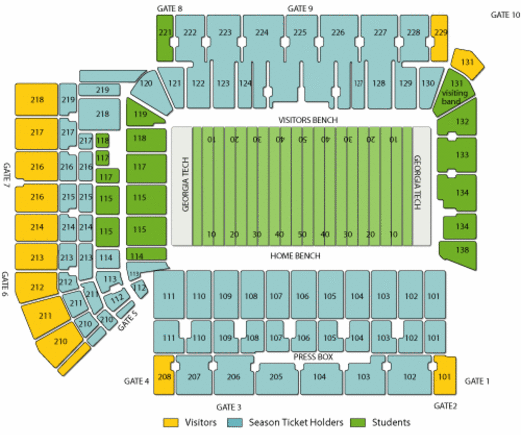
\includegraphics[width=\linewidth,natwidth=521,natheight=435]{stadium_diagram_updated.png}
  \caption{Bobby Stadium Stadium seating chart.}
  \label{fig:polygon}
\end{figure}

Our primary objective in this study is to minimize the pedestrian evacuation
time of the stadium and its surrounding area by attendees following a home
football game. We do this by taking a parametric approach, in which we explore
the effects of road closures, strategically placed guidance symbols
(i.e., signs), and the ``takeover" of certain intersections by law enforcement
in promoting an optimal result.

For purposes of this study, we define the system under investigation (SUI) as a
rectangular polygon (Fig. \ref{fig:polygon}) surrounding the stadium. To be clear,
the SUI is defined as the area outside the stadium, and not inclusive of the
stadium itself.

\begin{figure}[H]
  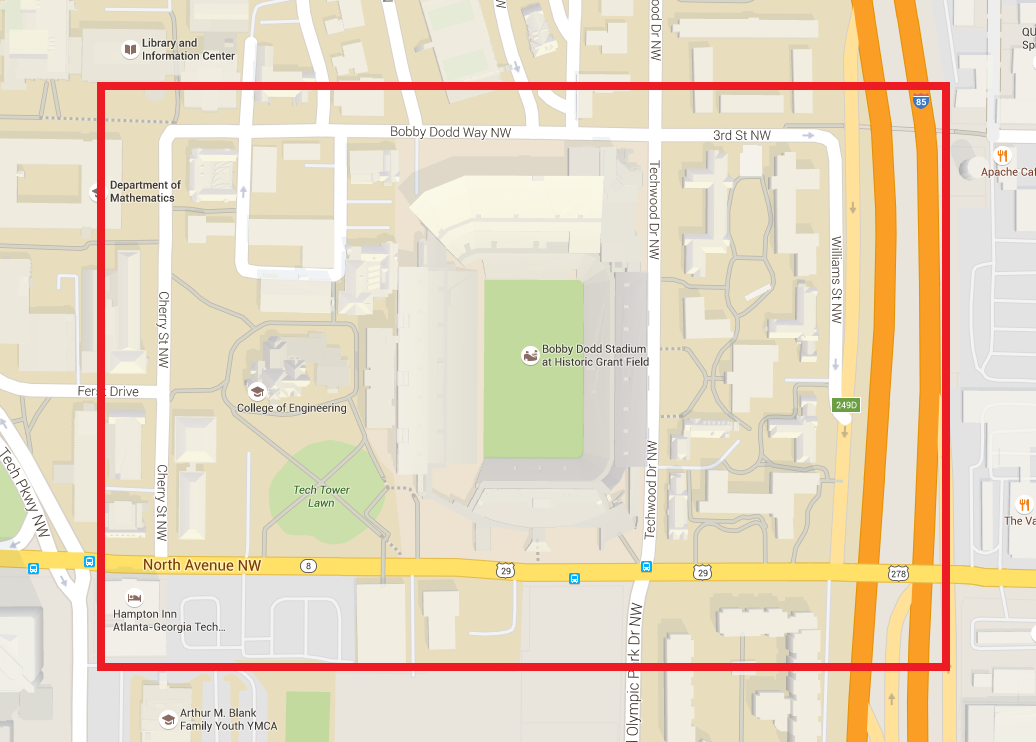
\includegraphics[width=\linewidth,natwidth=1036,natheight=742]{cropped_map.png}
  \caption{The system under investigation.}
  \label{fig:polygon}
\end{figure}

The stadium has 10 ``gates," which serve as ingress (pre-game) and egress
(post-game) sites.


\section{Related Work}
\label{sec:literature}

A variety of techniques have been used to model pedestrian movement. Cellular
automata, lattice gas, social force, fluid-dynamic, agent-based, game-theoretic,
and animal experimention-based approaches have been used
\cite{zheng2009modeling}. As noted by Zheng, Zhong, and Liu
\cite{zheng2009modeling}, models often encounter or attempt to model several
common phenomenoma: clogging, side-stepping, lane formation, and herding
behavior, among them.

These phenomena manifest themselves in different ways and at different
magnitudes depending on the system being modeled. In one of the early
explorations of 2D cellular automata for simulating traffic flow in the related
domain of vehicular traffic simulation, Biham and Middleton \cite{biham1992self}
note the presence of a sharp
\textit{jamming transition} in which all cars in the simulation transition from
moving at maximal speed to being stuck. Similar effects were noted in
simulations of bi-directional pedestrian movement, with Weifeng, Lizhong, and
Weicheng \cite{weifeng2003simulation} finding that as total pedestrian density
increases, a critical value is reached at which the system transitions into a
jammed state where only a few pedestrians are able to proceed.

In a slightly different take on the problem, Okazaki and Matsushita
\cite{okazaki1993study} modeled pedestrian evacuation using Coulomb's Law, with
actors magnetically moving toward their goals and away from obstacles that would
lead to collisions. In another application of equations of natural phenomena,
Helbing \cite{helbing1998fluid} derived fluid dynamic equations for explaining
the movement of pedestrian crowds, observing phenomena such as the development
of lanes, jamming, and crossing. Helbing \cite{helbing2000simulating} further
notes an explicit ``faster-is-slower" effect, in which attempting to move faster
results in a smaller average speed of leaving at high pedestrian density in
evacuation scenarios.

In a more recent study, Helbing et al. \cite{helbing2005self} use a
``social force" model, which states that pedestrians operate in some sense
automatically when reacting to obstacles and other pedestrians, applying
strategies that have been learned to be most effective over time. Several
suggestions are made to alleviate the three most common problems in pedestrian
crowds: counterflows, bottlenecks, and intersecting flows. The presence of
strategically placed obstacles are found to actually reduce these negative
phenomena, leading to improved flow.

Building on previous cellular automata-based models, Burstedde et al.
\cite{burstedde2001simulation} introduce a \textit{floor field}, a secondary
grid of cells which underlies the main grid and acts as a substitute for
pedestrian intelligence. These fields can be either static or dynamic, and are
capable of promoting the avoidance of jams, as well as simulating attractive
effects, in which pedestrians are more likely to follow in the paths of
pedestrians ahead of them.

Taking a more algorithmic approach, Fang et al. \cite{fang2011hierarchical} have
designed a modified ant colony optimization (ACO) algorithm for optimizing
pedestrian evacuation, seeking to minimize evacuation time, evacuation distance,
and congestion. Kemloh Wagoum, Seyfried, and Holl \cite{kemloh2012modeling}
utilize an observation principle approach in modeling pedestrian evacuation,
in which pedestrians first observe their environment and then make a final
decision on strategy based on obtained data.

There are several takeaways from the literature described above that have
potential applicability to the model at hand. First, on the topic of modeling
pedestrian walkways, several papers focused on either a single passageway,
enclosed areas with obstacles (walls, pillars, etc.), or evacuation from a
room with a single doorway. However, modeling walkways as a directed graph
\cite{fang2011hierarchical} seems feasible given the problem at hand, where
there are multiple pathways one can take to get to a single destination. In
papers where cellular automata was utilized, the median size of each cell on the
walkway was 0.4m\textsuperscript{2}
\cite{blue2001cellular,burstedde2001simulation,weifeng2003simulation}.

Second, on the topic of pedestrian modeling, multiple walking speed techniques
were used, ranging from a constant speed of 1 m/s \cite{weifeng2003simulation}
or 1.3 m/s \cite{burstedde2001simulation}, to using a distribution resembling a
step function \cite{blue2001cellular} or a Normal distribution
\cite{klupfel2005models}. In either distribution, the median walking speed was
also approximately 1.3 m/s. For reaction to stimuli, 0.3 seconds was utilized
\cite{burstedde2001simulation}, which was one time step in that particular
simulation. Incorporation of opportunistic side-stepping was done
\cite{blue2001cellular}, in addition to using least-cost algorithms for
establishing the path a pedestrian would like to take
\cite{fang2011hierarchical}. In the context of cellular automata, analyzing a
given pedestrian's cell's neighbors in either a 4-connected
\cite{weifeng2003simulation} or 8-connected fashion
\cite{burstedde2001simulation} to decide in which direction the pedestrian would
like to walk for the next time step was utilized. This, coupled with a dynamic
floor field \cite{burstedde2001simulation} to factor in long-distance forces,
could be utilized.

Finally, simulation execution practices were also gleaned. Care must be taken
to do parallel-based updating to avoid sequential updating from interfering with
underlying model execution \cite{blue2001cellular}. The practice of using
a deterministic model running with randomized initial conditions has precedent
\cite{biham1992self}. Finally, to achieve statistical significance, 20 runs per
configuration has been used \cite{blue2001cellular}.

\section{Conceptual Model}
For purposes of this simulation,
we define the . Our simulation is simplified by focusing only on
\textit{pedestrian} traffic, avoiding the inclusion of vehicular traffic. In
future studies, this could be included as an enhancement.

For the purposes of modeling egress, we choose to collapse
adjacent gates together, as it seems likely a similar approach would be taken
in reality.

For purposes of modeling egress, we assume pedestrian interarrival time at the
gate boundary is a homogenous stochastic process that follows a \textit{TODO: insert}
distribution. As pedestrians arrive at the gate boundary, and enter the system
under investi

\bibliography{template}{}
\bibliographystyle{plain}
\end{document}
